\documentclass[letterpaper,12pt]{article}
\usepackage[utf8]{inputenc}
\usepackage{charter}
\usepackage{geometry}
\usepackage{amsmath}
\usepackage{float}
\usepackage{graphicx}
\usepackage{subcaption}
\usepackage{amssymb}
\usepackage{adjustbox}
\usepackage{wrapfig} 
\usepackage{xcolor}
\usepackage{fancyhdr}
\usepackage{tabularx}
\usepackage{fancyhdr}
\usepackage{comment}

\geometry{top=2cm, bottom=2cm, left=2cm, right= 2cm} %%margen
\graphicspath{{images/}}
\parindent=0pt

\begin{document}
%%para contador y eso
\thispagestyle{empty}
\newpage
\setcounter{page}{1}
\pagestyle{headings}
%%%%%%%%%%%%%%%%%%%%%%%%%%%%%%%%%%%%%%%%%%%%%%%%%%%%%%%%%%%%%%%%%%%%%%%%%%%%
\begin{sloppypar} 
    %%%portadita
\begin{titlepage}
    \fancyhead{R}{
    
\includegraphics[width=0.1\linewidth]{logoUV.png}
    }
    \hspace{2.5cm}
    {\bfseries\LARGE Universidad Veracruzana \par}
    \hspace{2cm}
    {\scshape\Large Facultad de Ingeniería Eléctrica y Electrónica \par}
    \begin{center}
        \vspace{5cm}
        \begin{figure}[H]
            \centering 
            
\includegraphics[width=0.9\textwidth]{PORTADA.png}
        \end{figure}
        \vspace{2cm}
        {\itshape\Large E12 - STP 2 \par}
        {\large Lara Xocuis Martha Denisse \par}
        {\large S22002213 \par}
        \vfill
        {\Large \today \par}
    \end{center}
    
\end{titlepage} 

%%%%%%%%%%%%%%%%%%%%%%TOPOLOGÍA%%%%%%%%%%%%%%%%%%%%%%
\section{Topología de Red}
\begin{figure}[H]
    \centering 
    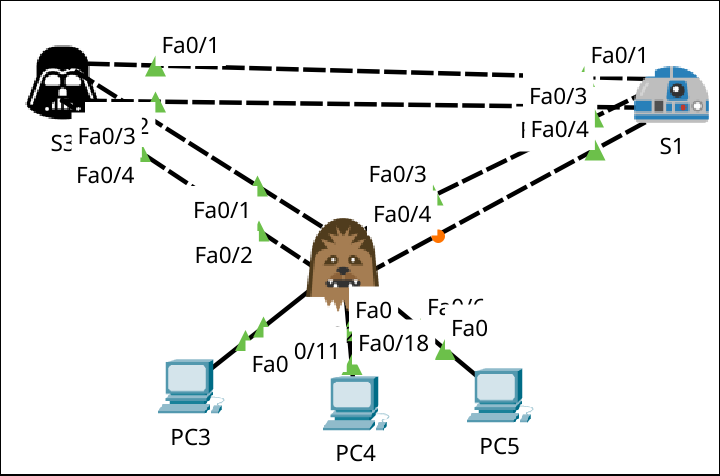
\includegraphics[width=0.8\textwidth]{topo.png}
\end{figure}

\section{Información de las VLANs}
\subsection{show spanning-tree}
\begin{figure}[H]
    \centering 
    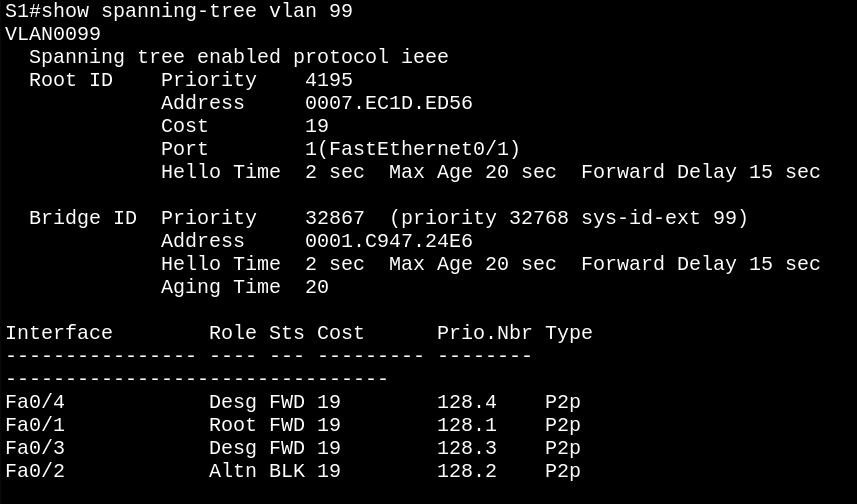
\includegraphics[width=0.6\textwidth]{spaningtre1.png}
    \vspace{0.3cm}\\ 
    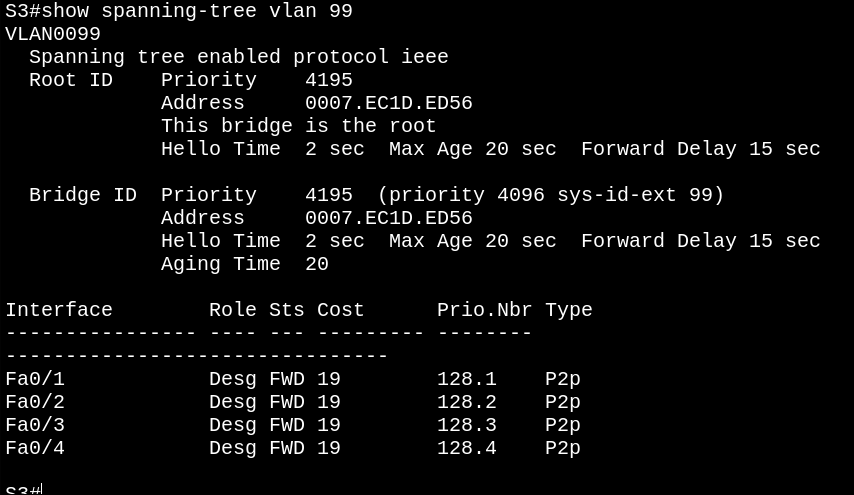
\includegraphics[width=0.6\textwidth]{spa2.png}
    \vspace{0.3cm}\\ 
    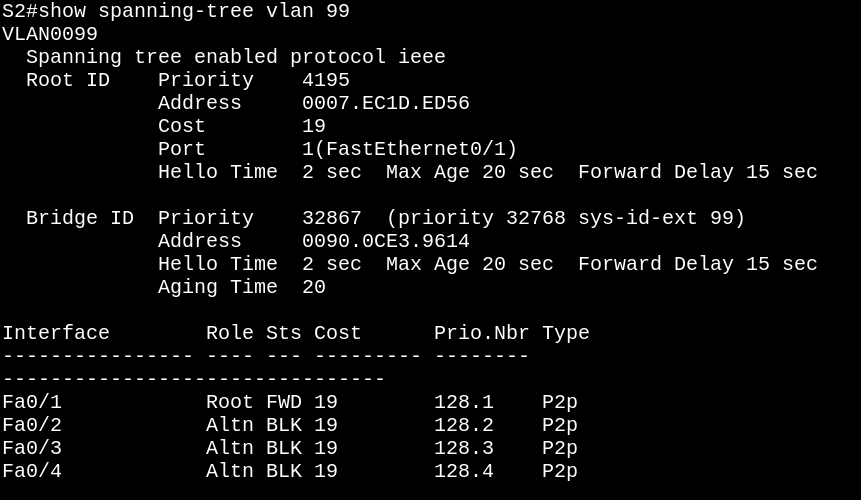
\includegraphics[width=0.6\textwidth]{s2spa.png}
\end{figure}
\subsection{show vlan brief}
\begin{figure}[H]
    \centering
    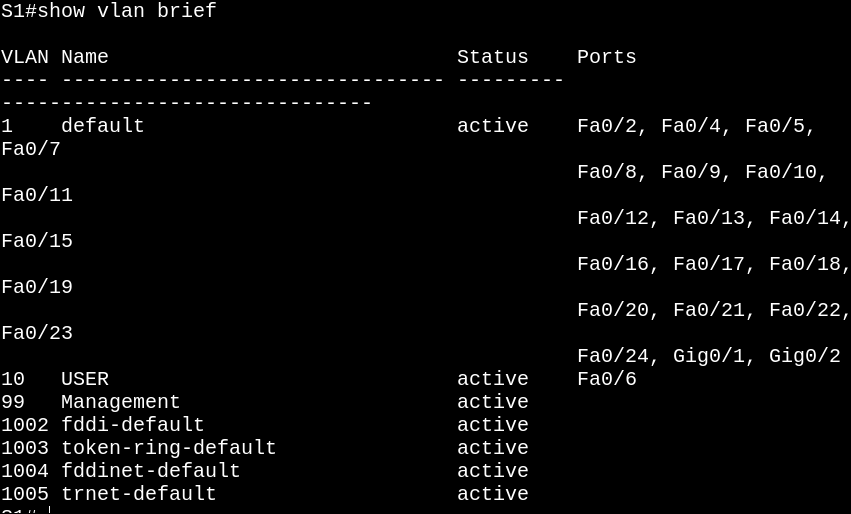
\includegraphics[width=0.6\textwidth]{vlanbrief1.png}
    \vspace{0.3cm}\\ 
    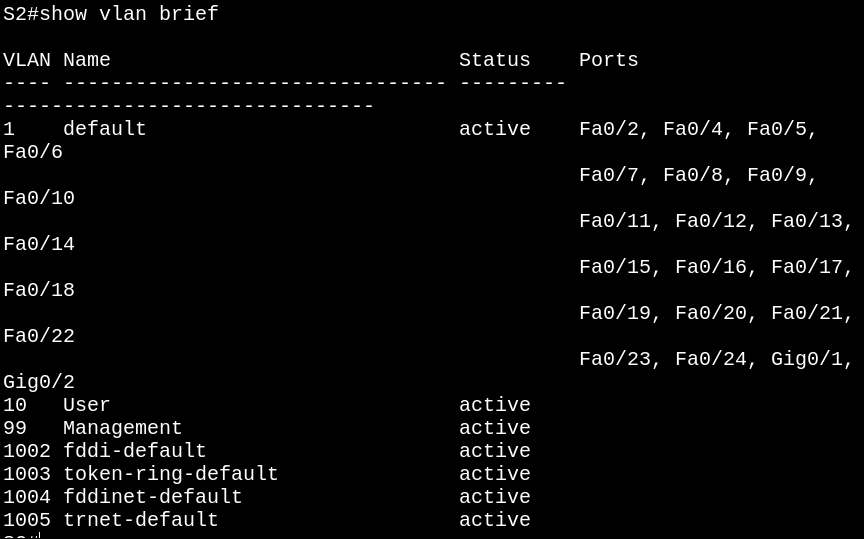
\includegraphics[width=0.6\textwidth]{vlanbrief2.png}
    \vspace{0.3cm}\\ 
    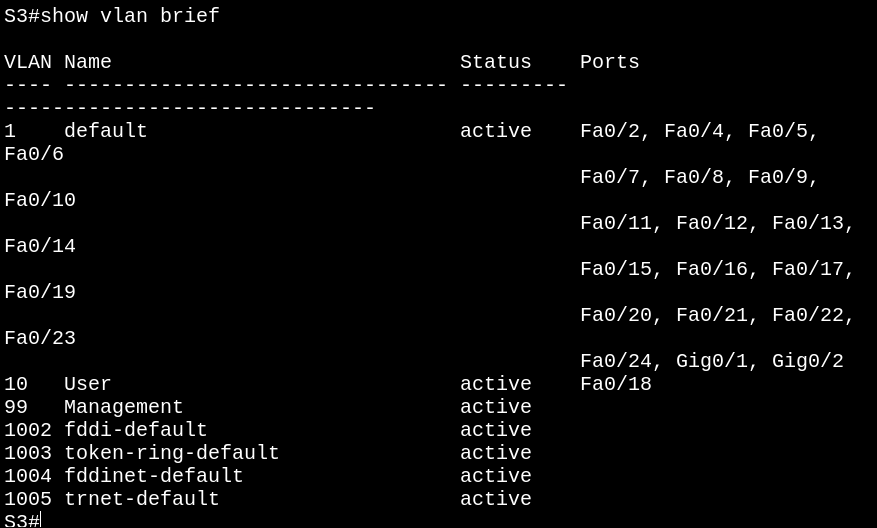
\includegraphics[width=0.6\textwidth]{vlanbrief3.png}
\end{figure}
\newpage
\subsection{show interface trunk}
\begin{figure}[H]
    \centering
    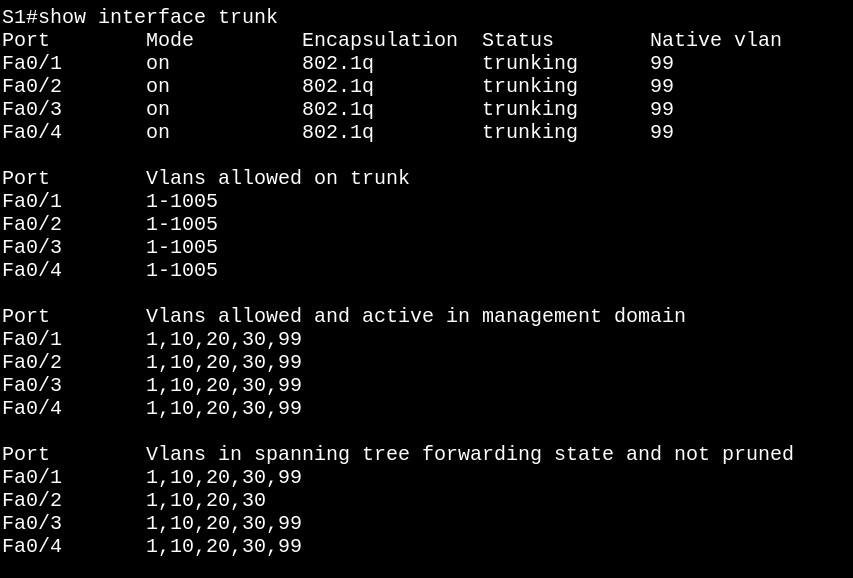
\includegraphics[width=0.6\textwidth]{trunk1.png}
    \vspace{0.3cm}\\ 
    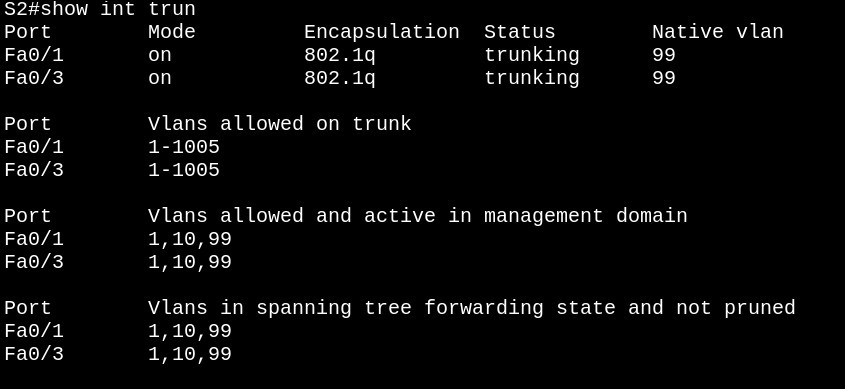
\includegraphics[width=0.6\textwidth]{trunk2.png}
    \vspace{0.3cm}\\ 
    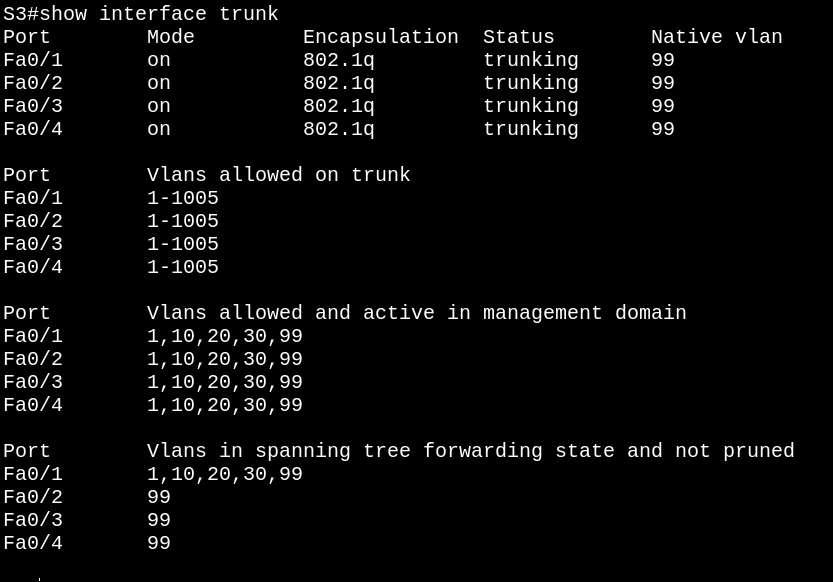
\includegraphics[width=0.6\textwidth]{trunk3.png}
\end{figure}
\subsection{show vtp status}
\begin{figure}[H]
    \centering
    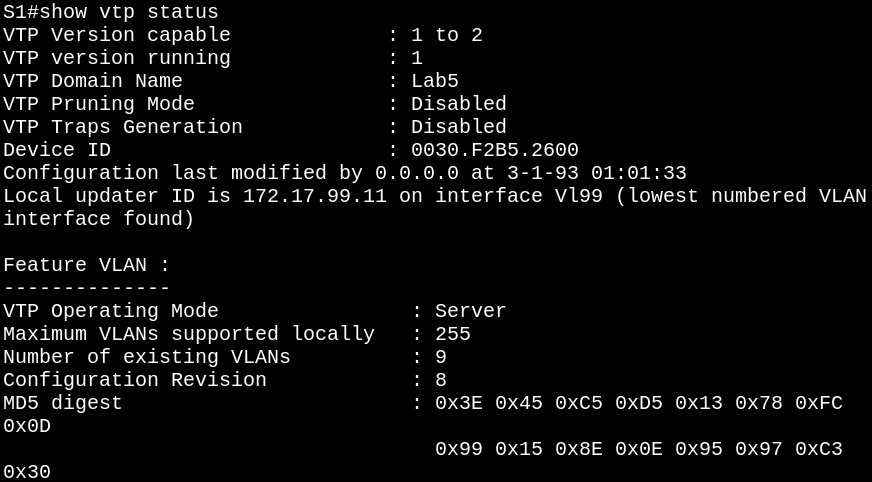
\includegraphics[width=0.6\textwidth]{vtp1.png}
    \vspace{0.3cm}\\ 
    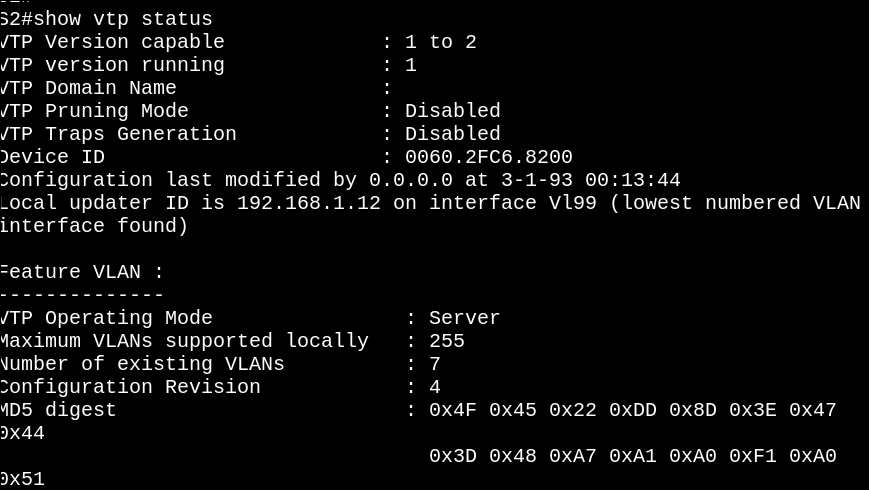
\includegraphics[width=0.6\textwidth]{vtp2.png}
    \vspace{0.3cm}\\ 
    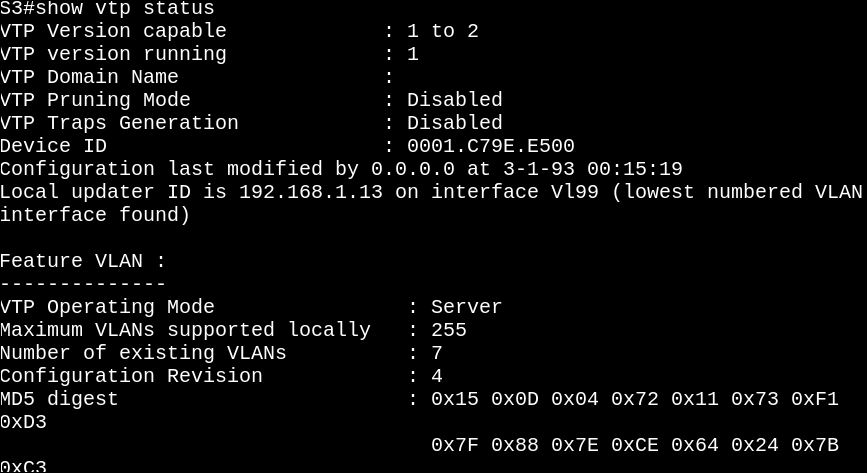
\includegraphics[width=0.6\textwidth]{vtp3.png}
\end{figure}
\newpage
\subsection{Asignaciones - Tablas}
\subsubsection{SWITCH S1}
    \begin{center}
        \begin{tabular}{|c|c|c|c|c|} \hline
            %Finalmente realiza un tabla de todos los swithces por cada VLAN con respectivos roles, estados y costo de los puertos y quién es el puente raíz.%
        VLAN & ROL & ESTADO & COSTO PUERTOS & RAIZ \\ \hline
        01 & Desg & FWD & 19 & Si  \\ \hline
        10 & Desg & FWD & 19 & Si \\ \hline 
        20 & Desg & FWD & 19 & Si \\ \hline
        30 & Desg & FWD & 19 & Si \\ \hline
        99 & Desg, Altn & BLK, FWD & 19 & No \\ \hline
        \end{tabular}   
    \end{center}
\subsubsection{SWITCH S2}
\begin{center}
    \begin{tabular}{|c|c|c|c|c|} \hline
        %Finalmente realiza un tabla de todos los swithces por cada VLAN con respectivos roles, estados y costo de los puertos y quién es el puente raíz.%
    VLAN & ROL & ESTADO & COSTO PUERTOS & RAIZ \\ \hline
    01 & Desg, Root, Altn & FWD, BLK & 19 & No  \\ \hline
    10 & Desg, Root, Altn & FWD, BLK & 19 & No \\ \hline 
    20 & Desg, Root, Altn & FWD, BLK & 19 & No \\ \hline
    30 & Desg, Root, Altn & FWD, BLK & 19 & No \\ \hline
    99 & Root, Altn & BLK, FWD & 19 & No \\ \hline
    \end{tabular}   
\end{center}

\subsubsection{SWITCH S3}
\begin{center}
    \begin{tabular}{|c|c|c|c|c|} \hline
        %Finalmente realiza un tabla de todos los swithces por cada VLAN con respectivos roles, estados y costo de los puertos y quién es el puente raíz.%
    VLAN & ROL & ESTADO & COSTO PUERTOS & RAIZ \\ \hline
    01 & Root, Altn & FWD, BLK & 19 & No  \\ \hline
    10 & Root, Altn & FWD, BLK & 19 & No \\ \hline 
    20 & Root, Altn & FWD, BLK & 19 & No \\ \hline
    30 & Root, Altn & FWD, BLK & 19 & No \\ \hline
    99 & Desg & FWD & 19 & Si \\ \hline
    \end{tabular}   
\end{center}

\end{sloppypar}
\end{document}